% *********************************************************************
% © 2016–2025 Jeremy Sylvestre
%
% Permission is granted to copy, distribute and/or modify this document
% under the terms of the GNU Free Documentation License, Version 1.3 or
% any later version published by the Free Software Foundation; with no
% Invariant Sections, no Front-Cover Texts, and no Back-Cover Texts. A
% copy of the license is included in the appendix entitled “GNU Free
% Documentation License” that appears in the output document of this
% PreTeXt source code. All trademarks™ are the registered® marks of
% their respective owners.
%
% *********************************************************************
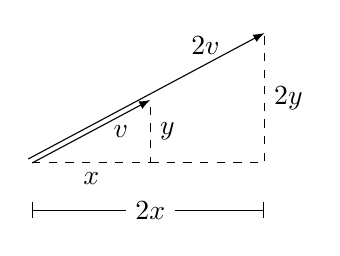
\begin{tikzpicture}[
	point/.style={circle,draw,very thin,fill,inner sep=0pt,minimum size=4pt},
	vector/.style={-latex},
]
	\coordinate (o) at (0,0);
	\coordinate (oshift) at (-0.05,0.05);
	\coordinate (v)   at (1.5,0.8);
	\coordinate (vx)  at (1.5,0);
	\coordinate (v2)  at (2.95,1.65);
	\coordinate (vx2) at (2.95,0);

	\draw[vector] (o) to node[below,near end] {$\uvec{v}$} (v);
	\draw[vector] (oshift) to node[above,near end] {$2\uvec{v}$} (v2);
	\draw[dashed] (o) to node[below] {$\change{x}$} (vx) to node[right] {$\change{y}$} (v);
	\draw[dashed] (vx) to (vx2) to node[right] {$2 \change{y}$} (v2);
	\node (dx) at (1.5,-0.6) {$2 \change{x}$};
	\draw[|-] (0,-0.6) to (dx);
	\draw[-|] (dx) to (2.95,-0.6);
	% \draw (0,-0.75) to (ddx.west);
	% \draw (ddx.east) to (3,-0.75);
	% \draw (0,-0.65) to (0,-0.85);
	% \draw (3,-0.65) to (3,-0.85);
\end{tikzpicture}
